\documentclass{article}%
\usepackage[T1]{fontenc}%
\usepackage[utf8]{inputenc}%
\usepackage{lmodern}%
\usepackage{textcomp}%
\usepackage{lastpage}%
\usepackage[head=40pt,margin=0.5in,bottom=0.6in]{geometry}%
\usepackage{graphicx}%
%
\title{\textbf{Costa Rica apoya iniciativa para investigar a Nicolás Maduro ante CPI}}%
\author{El Nacional Web}%
\date{16/10/2018}%
%
\begin{document}%
\normalsize%
\maketitle%
\textbf{URL: }%
http://www.el{-}nacional.com/noticias/latinoamerica/costa{-}rica{-}apoya{-}iniciativa{-}para{-}investigar{-}nicolas{-}maduro{-}ante{-}cpi\_256076\newline%
%
\textbf{Periodico: }%
EN, %
ID: %
256076, %
Seccion: %
Latinoamérica\newline%
%
\textbf{Palabras Claves: }%
NO\_TIENE\newline%
%
\textbf{Derecho: }%
CONTEXTO, %
Otros Derechos: %
18, %
Sub Derechos: %
\newline%
%
\textbf{EP: }%
NO\newline%
\newline%
%
\textbf{\textit{La información fue suministrada mediante un comunicado este martes}}%
\newline%
\newline%
%
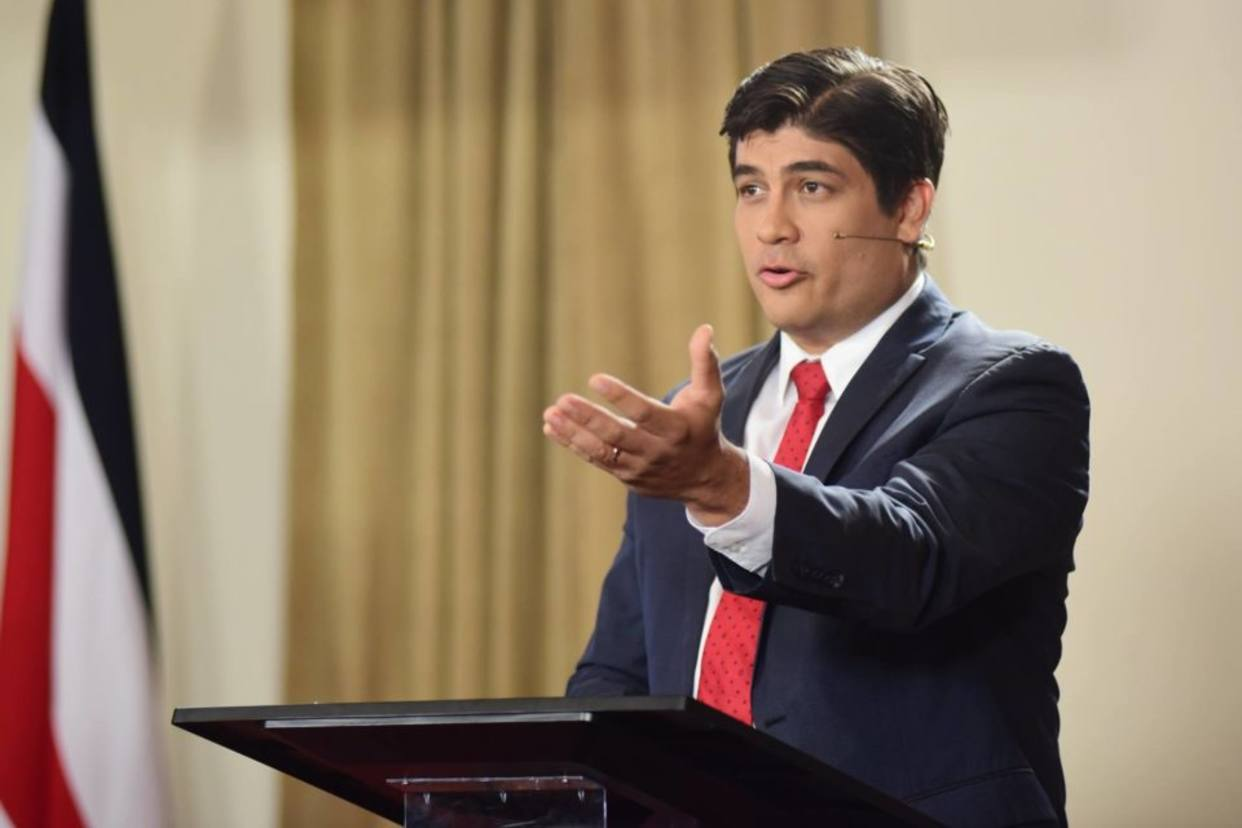
\includegraphics[width=300px]{104.jpg}%
\newline%
%
Carlos Alvarado, presidente de Costa Rica, anunció que su país apoya~ la iniciativa de Argentina, Canadá, Chile, Colombia, Paraguay y Perú para que la Corte Penal Internacional investigue la posible comisión de crímenes de lesa humanidad~por el gobierno de Nicolás Maduro.%
\newline%
%
“En seguimiento a su histórica lucha contra la impunidad, Costa Rica apoya las gestiones, presentadas el 26 de setiembre del 2018, por seis países de América, con base en el artículo 14.2 del Estatuto de Roma, en el que le solicitan a la Fiscalía se inicie una investigación sobre la posible comisión de crímenes de lesa humanidad, que pudieran haber ocurrido a partir del 12 de febrero de 2014.”, afirmó el mandatario.%
\newline%
%
Costa Rica confía en la independencia~de la corte para investigar y tomar las medidas necesarias, según el comunicado publicado en el Ministerio de Relaciones Exteriores y Culto.%
\newline%
%
Hizo~un llamado a las autoridades de Venezuela para que cumplan con las obligaciones internacionales adquiridas al acceder a los intrumentos jurídicos internacionales de los DD HH.%
\newline%
%
El Estado costarricense indicó que continuará los~foros multilaterales y canales diplomáticos~para contribuir a la superación de la crisis venezolana, mediante una salida pacífica y negociada.%
\newline%
%
Con información del~Ministerio de Relaciones Exteriores y Culto%
\newline%
%
\end{document}